\solutionset

\begin{enumerate}

\item {\bf A Simple Protostellar Evolution Model.}

\begin{enumerate}

\item The star is a polytrope, and for a polytrope of index $n$ the gravitational energy is (e.g., see \citealt{kippenhahn94a})
\begin{displaymath}
\mathcal{W} = -\frac{3}{5-n} \frac{G M^2}{R}.
\end{displaymath}
The virial theorem tells us that the thermal energy is half the absolute value of the potential energy, so
\begin{displaymath}
\mathcal{T} = \frac{3}{2(5-n)} \frac{G M^2}{R}.
\end{displaymath}
Finally, the change in internal energy associated with dissociation, ionization, and deuterium burning is $(\psi_I  + \psi_M - \psi_D) M$. Note the opposite signs: $\psi_I$ and $\psi_M$ are positive, meaning that the final state (ionized, atomic) is higher energy than the initial one, while $\Psi_D$ is negative, indicating that the final state (all the deuterium converted to He) is a lower energy state than the initial one. Putting this all together, the total energy of the star is
\begin{displaymath}
\mathcal{E} = -\frac{3}{2(5-n)} \frac{G M^2}{R} + (\psi_I  + \psi_M - \psi_D) M.
\end{displaymath}

\item First we can compute the time rate of change of the star's energy,
\begin{displaymath}
\dot{\mathcal{E}} = \frac{3}{2(5-n)} \frac{GM}{R} \left(M\frac{\dot{R}}{R} - 2\dot{M}\right) + (\psi_I + \psi_M-\psi_D) \dot{M}.
\end{displaymath}
Now consider conservation of energy. The star's luminosity $L$ represents the rate of change of the energy "at infinity", i.e., the energy removed from the system. Since the total energy of the star plus infinity must remain constant, we require that $\dot{\mathcal{E}} + L = 0$. Writing down this condition and solving for $\dot{R}$, we obtain
\begin{displaymath}
\dot{R} = 2 R \frac{\dot{M}}{M} - \frac{2(5-n)}{3} \frac{R^2}{G M^2}\left[(\psi_I+\psi_M-\psi_D) \dot{M}+L\right]
\end{displaymath}
It is convenient to divide through by $\dot{M}$ in order to recast this as an equation for the evolution of $R$ with $M$:
\begin{displaymath}
\frac{dR}{dM} = 2 \frac{R}{M} - \frac{2(5-n)}{3} \frac{R^2}{G M^2}\left(\psi_I+\psi_M-\psi_D+\frac{L}{\dot{M}}\right).
\end{displaymath}
If we further divide by $R/M$ on both sides, we obtain
\begin{displaymath}
\frac{d\ln R}{d\ln M} = 2 - \frac{2(5-n)}{3} \frac{R}{G M}\left(\psi_I+\psi_M-\psi_D+\frac{L}{\dot{M}}\right).
\end{displaymath}
Next, we must compute the total luminosity, which contains contributions from the star's intrinsic, internal luminosity, and from the accretion luminosity. Since the star is on the Hayashi track, we can compute the intrinsic luminosity by taking its effective temperature to be fixed at $T_H$. Thus the total luminosity is
\begin{displaymath}
L = L_{\rm acc} + L_H = f_{\rm acc} \frac{G M \dot{M}}{R} + 4\pi R^2 \sigma T_H^4.
\end{displaymath}
Substituting this in, we have
\begin{displaymath}
\frac{d\ln R}{d\ln M} = 2 - \frac{2(5-n)}{3} \left[f_{\rm acc} + \left(\frac{R}{G M}\right)\left(\psi_I+\psi_M -\psi_D + \frac{4\pi R^2\sigma T_H^4}{\dot{M}}\right)\right].
\end{displaymath}
This is our final evolution equation.

\item The ODE can be integrated by standard techniques. Below is an example python program to do so, and plot the result:
\begin{verbatim}
import numpy as np
import matplotlib.pyplot as plt
from scipy.integrate import odeint

# Define some constants in cgs
G = 6.67e-8
eV = 1.6e-12
amu = 1.66e-24
sigma = 5.67e-5
Msun = 1.99e33
Rsun = 6.96e10
Lsun = 3.83e33
yr = 365.25*24.*3600.

# Problem parameters
psiI = 13.6*eV/amu
psiM = 2.2*eV/amu
psiD = 100*eV/amu
tH = 3500.0

# Default parameters
n = 1.5
facc = 0.75
Mdot = 1e-5*Msun/yr

# Define the derivative function
def dlnRdlnM(lnR, lnM, n=n, facc=facc, Mdot=Mdot):
    R = np.exp(lnR)
    M = np.exp(lnM)
    return(2.0-2.0*(5.0-n)/3.0 *
           (facc+(R/(G*M))*
            (psiI+psiM-psiD+
             4.0*np.pi*R**2*sigma*tH**4/Mdot)))

# Integrate
lnM = np.log(np.logspace(-2, 0, 500)*Msun)
lnR = odeint(dlnRdlnM, np.log(2.5*Rsun), lnM,
             args=(n, facc, Mdot))
R = np.exp(lnR[:,0])
M = np.exp(lnM)
             
# Get luminosity
L = facc*G*M*Mdot/R + 4.0*np.pi*R**2*sigma*tH**4

# Plot radius
p1,=plt.plot(M/Msun, R/Rsun, 'b', lw=2)
plt.xscale('log')
plt.xlabel(r'$M/M_\odot$')
plt.ylabel(r'$R/R_\odot$')

# Plot luminosity
plt.twinx()
p2,=plt.plot(M/Msun, L/Lsun, 'r', lw=2)
plt.ylabel(r'$L/L_\odot$')
plt.legend([p1,p2], ['Radius', 'Luminosity'],
           loc='lower right')
\end{verbatim}
\begin{marginfigure}
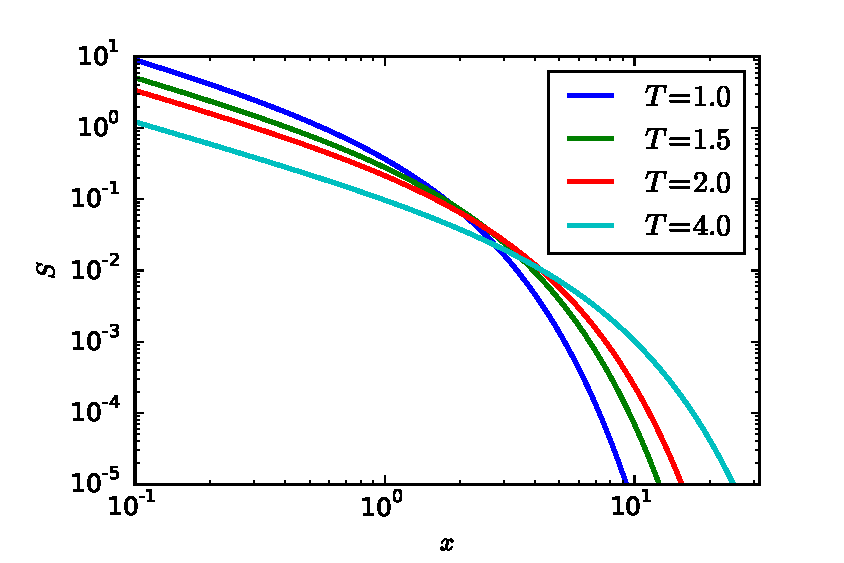
\includegraphics[width=\linewidth]{hw4sol1}
\caption[Solution to problem set~\thesolutionset, problem~\theenumi\theenumii]{
\label{fig:hw4sol1}
Radius (blue) and luminosity (red) for the simple protostellar evolution model.
}
\end{marginfigure}
The resulting output is shown as Figure \ref{fig:hw4sol1}. Note that the radius is too large by a factor of $\sim 3$ compared to more sophisticated models, mainly due to the incorrect assumption that all the accreted deuterium burns as quickly as it accretes. In reality the D luminosity should be significantly lower, because D burning lasts longer than accretion.

\item This problem can be solved using the same basic structure as the previous part. The derivative of radius with respect to mass now becomes
\begin{eqnarray*}
\frac{d\ln R}{d\ln M} & = & 2 - \frac{2(5-n)}{3} \left[f_{\rm acc} + \left(\frac{R}{G M}\right) \cdot \right.
\\
& & \qquad \left.\left(\psi_I+\psi_M -\psi_D + \frac{\max[4\pi R^2\sigma T_H^4, \lsun (M/\msun)^3]}{\dot{M}}\right)\right].
\end{eqnarray*}
This can be integrated via a simple python program as in the previous part:
\begin{verbatim}
# Define the derivative function for the second part
def dlnRdlnM2(lnR, lnM, n=n, facc=facc, Mdot=Mdot):
    R = np.exp(lnR)
    M = np.exp(lnM)
    LH = 4.0*np.pi*R**2*sigma*tH**4
    Lstar = Lsun*(M/Msun)**3
    return(2.0-2.0*(5.0-n)/3.0 *
           (facc+(R/(G*M))*
            (psiI+psiM-psiD+np.maximum(Lstar,LH)/Mdot)))

# Integrate
Mdot2 = 1.0e-4*Msun/yr
lnM2 = np.log(np.logspace(-2, np.log10(50), 500)*Msun)
lnR2 = odeint(dlnRdlnM2, np.log(2.5*Rsun), lnM2,
              args=(3.0, facc, Mdot2))
R2 = np.exp(lnR2[:,0])
M2 = np.exp(lnM2)

# Get luminosity
L2 = facc*G*M*Mdot/R + np.maximum(
    4.0*np.pi*R2**2*sigma*tH**4,
    Lsun*(M2/Msun)**3)

# Plot radius
plt.clf()
p1,=plt.plot(M2/Msun, R2/Rsun, 'b', lw=2)
plt.xlabel(r'$M/M_\odot$')
plt.ylabel(r'$R/R_\odot$')

# Plot luminosity
plt.twinx()
p2,=plt.plot(M2/Msun, L2/Lsun, 'r', lw=2)
plt.ylabel(r'$L/L_\odot$')
plt.yscale('log')
plt.xlim([0,50])
plt.legend([p1,p2], ['Radius', 'Luminosity'], 
           loc='center right')
\end{verbatim}
\begin{marginfigure}
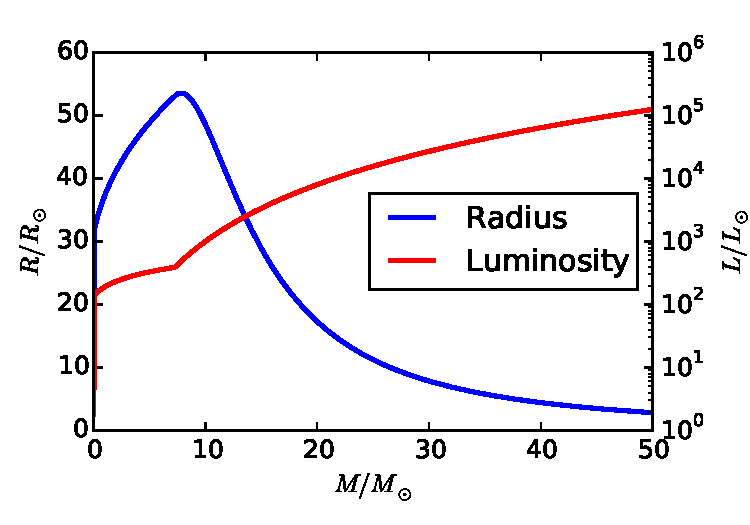
\includegraphics[width=\linewidth]{hw4sol2}
\caption[Solution to problem set~\thesolutionset, problem~\theenumi\theenumii]{
\label{fig:hw4sol2}
Radius (blue) and luminosity (red) for the simple protostellar evolution model for a massive star.
}
\end{marginfigure}
The resulting output is shown as Figure \ref{fig:hw4sol2}.

\end{enumerate}

\item \textbf{Self-Similar Viscous Disks.}

\begin{enumerate}

\item First let us plug in the given form for $\nu$:
\begin{displaymath}
\frac{\partial\Sigma}{\partial t} = \frac{\nu_1}{\varpi_1} \frac{3}{\varpi} \frac{\partial}{\partial \varpi} \left[\varpi^{1/2} \frac{\partial}{\partial \varpi} \left(\Sigma \varpi^{3/2}\right)\right].
\end{displaymath}
Next, let's make the change of variables $\varpi = \varpi_1 x$. Note that this also implies that $\partial /\partial \varpi = (1/\varpi_1) \partial/\partial x$. With this change, we have
\begin{displaymath}
\frac{\partial\Sigma}{\partial t} = \frac{\nu_1}{\varpi_1^2} \frac{3}{x} \frac{\partial}{\partial x} \left[x^{1/2} \frac{\partial}{\partial x} \left(\Sigma x^{3/2}\right)\right].
\end{displaymath}
The third step is to make the change of variables $t = T t_s$, $\partial/\partial t = (1/t_s) \partial/\partial T$, then simplify:
\begin{eqnarray*}
\frac{3\nu_1}{\varpi_1^2} \frac{\partial\Sigma}{\partial T} & = & \frac{\nu_1}{\varpi_1^2} \frac{3}{x} \frac{\partial}{\partial x} \left[x^{1/2} \frac{\partial}{\partial x} \left(\Sigma x^{3/2}\right)\right] \\
\frac{\partial\Sigma}{\partial T} & = & \frac{1}{x} \frac{\partial}{\partial x} \left[x^{1/2} \frac{\partial}{\partial x} \left(\Sigma x^{3/2}\right)\right].
\end{eqnarray*}
The last step is to substitute in for $\Sigma$, which is trivial:
\begin{displaymath}
\frac{\partial S}{\partial T} = \frac{1}{x} \frac{\partial}{\partial x} \left[x^{1/2} \frac{\partial}{\partial x} \left(S x^{3/2}\right)\right].
\end{displaymath}
This is the non-dimensional equation we wanted.

\item We can show that the given form is a solution simply by plugging in the equivalent non-dimensional solution for $S$, which is
\begin{displaymath}
S = \frac{e^{-x/T}}{x T^{3/2}}.
\end{displaymath}
Plugging this into the two sides of the non-dimensional equation, we get
\begin{eqnarray*}
\frac{\partial S}{\partial T} & = & \left(\frac{2x - 3 T}{2 x T^{7/2}}\right) e^{-x/T} \\
\frac{1}{x} \frac{\partial}{\partial x} \left[x^{1/2} \frac{\partial}{\partial x} \left(S x^{3/2}\right)\right]
& = & 
\frac{1}{x} \frac{\partial}{\partial x} \left[\left(\frac{T-2x}{2 T^{5/2}}\right) e^{-x/T}\right] \\
& = & \left(\frac{2x - 3 T}{2 x T^{7/2}}\right) e^{-x/T}.
\end{eqnarray*}
Since the two sides match, this suffices to show that $S=e^{-x/T}/(x T^{3/2})$ is a solution. Since we have made no assumptions about the value of $\Sigma_1$ in this argument, we are free to choose its value to be whatever we want. In particular, if we choose $\Sigma_1 = C/3\pi \nu_1$, then we immediately obtain the solution
\begin{displaymath}
\Sigma = \left(\frac{C}{3\pi \nu_1}\right)\frac{1}{x T^{3/2}} e^{-x/T}.
\end{displaymath}

\item The disk mass is simply given by
\begin{eqnarray*}
M_d & = & \int_0^\infty 2\pi \varpi \Sigma \, d\varpi \\
& = & \varpi_1^2 \int_0^\infty 2\pi x \Sigma \, dx \\
& = & \left(\frac{2 C \varpi_1^2}{3 \nu_1}\right) \frac{1}{T^{3/2}} \int_0^\infty e^{-x/T} \, dx \\
& = & \frac{2 C \varpi_1^2}{3 \nu_1 T^{1/2}} \\
& = & 2 C t_s \left(\frac{t}{t_s}\right)^{-1/2}.
\end{eqnarray*}
The time rate of change of the disk mass is just
\begin{displaymath}
\dot{M}_d = -C \left(\frac{t}{t_s}\right)^{-3/2}.
\end{displaymath}
Looking at the equation, and noting that $C$ has units of mass per time, it is clear that $C$ controls the accretion rate of the disk onto the point mass in the center.

\begin{marginfigure}
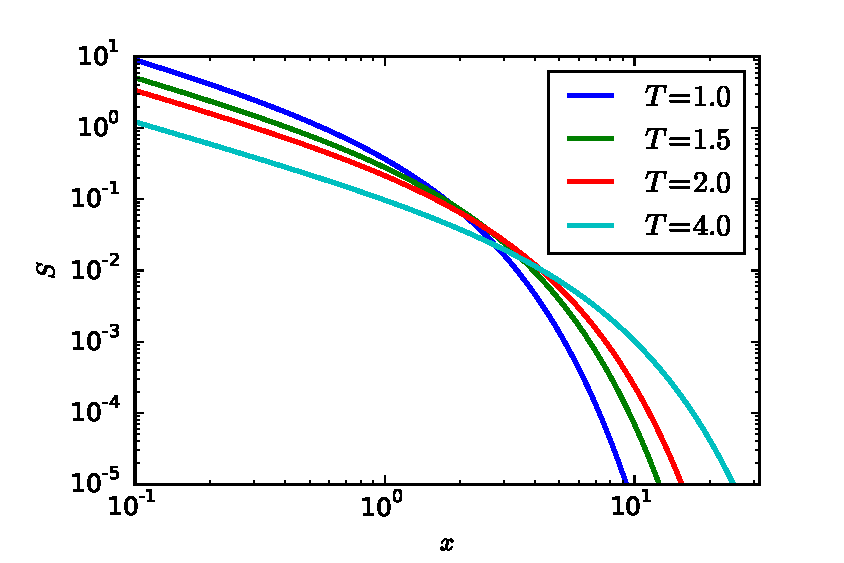
\includegraphics[width=\linewidth]{hw4sol3}
\caption[Solution to problem set~\thesolutionset, problem~\theenumi\theenumii]{
\label{fig:hw4sol3}
$S$ versus $x$ at dimensionless times $T=1, 1.5, 2$, and 4.
}
\end{marginfigure}
\item Figure \ref{fig:hw4sol3} shows the required plot. We see that the disk surface density profile follows $S\propto x^{-1}$ for $x<T$, and is exponentially truncated at $x>T$. We can think of the inner part as the ``main disk", and the outer part as the material pushed outward by viscosity in order to compensate for the angular momentum lost as other gas moves inwards. As time passes, the inner, main disk drains onto the star, and its surface density decreases. At the same time, the outer, exponentially truncated segment of the disk grows to larger and larger radii as more and more angular momentum is extracted from the inner disk.

\end{enumerate}

\item \textbf{A Simple T Tauri Disk Model.}

\begin{enumerate}

\item The disk interior is optically thick, so the vertical radiation flux $F$ is given by the diffusion approximation:
\begin{displaymath}
F = \frac{c}{3\kappa\rho} \frac{d}{dz} E = \frac{ca}{3\kappa\rho} \frac{d}{dz} (T^4) = \frac{4 \sigma}{3\kappa\rho}  \frac{d}{dz} (T^4)
\end{displaymath}
where $E$ is the radiation energy density and $T$ is the gas temperature. In thermal equilibrium the flux does not vary with $z$, so we can re-arrange this equation and integrate from the midplane at $z=0$ to the surface at $z=z_s$:
\begin{eqnarray*}
F \int_0^{z_s} \rho \, dz & = & \frac{4\sigma}{3\kappa} \int_{T_m}^{T_s} \frac{d}{dz} T^4 \, dz \\
F \frac{\Sigma}{2} & = & \frac{4\sigma}{3\kappa} \left(T_m^4 - T_s^4\right) \\
F & \approx & \frac{8\sigma}{3\kappa\Sigma} T_m^4,
\end{eqnarray*}
where the factor of 2 in the denominator on the LHS in the second step comes from the fact that $\Sigma$ is the column density of the entire disk, and we integrated over only half of it. In the third step we assumed that $T_m^4 \gg T_s^4$, which will be true for any optically thick disk. Note that this is the flux carried away from the disk midplane in both the $+z$ and $-z$ directions -- formally the flux changes direction discontinuously at $z=0$ in this simple model, so the total flux leaving the midplane is twice this value. If the disk radiates as a blackbody, the radiation flux per unit area leaving each side of the disk surface is $\sigma T_s^4$, and this must balance the flux that is transported upward through the disk by diffusion. Thus we have
\begin{displaymath}
\frac{8\sigma}{3\kappa\Sigma} T_m^4 \approx \sigma T_s^4,
\end{displaymath}
where the expressions on either side of the equality represent the fluxes in either the $+z$ or $-z$ directions either; the total fluxes are a factor of 2 greater, but the factors of 2 obviously cancel. Solving for $T_m$ gives the desired result:
\begin{displaymath}
T_m \approx \left(\frac{3}{8}\kappa\Sigma\right)^{1/4} T_s.
\end{displaymath}

\item Equating the dissipation rate $F_d$ per unit area with the radiation rate per unit area $\sigma T_s^4$ 
\begin{eqnarray*}
\sigma T_s ^4 & = &\frac{9}{8} \nu \Sigma \Omega^2\\
T_s & = & \left(\frac{9}{8}\frac{\nu\Sigma\Omega^2}{\sigma}\right)^{1/4} \\
& = & \left(\frac{9}{8} \alpha \frac{c_s^2 \Sigma \Omega}{\sigma}\right)^{1/4}
\end{eqnarray*}
In turn, plugging this into the relation we just derived between the surface and midplane temperatures gives
\begin{eqnarray*}
T_m & \approx & \left(\frac{27}{64} \frac{\nu \kappa \Sigma^2 \Omega^2}{\sigma}\right)^{1/4} \\
& \approx & \left(\frac{27}{64} \frac{\alpha \kappa c_s^2 \Sigma^2 \Omega}{\sigma}\right)^{1/4}
\end{eqnarray*}
Substituting $c_s^2 = k_B T_m / \mu m_{\rm H}$, where $\mu$ is the mean particle mass in units of $m_{\rm H}$, and solving for $T_m$ gives
\begin{displaymath}
T_m \approx
\left(\frac{27}{64} \frac{\alpha k_B \kappa \Sigma^2 \Omega}{\sigma \mu m_{\rm H}}\right)^{1/3}.
\end{displaymath}
Note that it makes much more sense to compute $c_s$ from the midplane temperature than from the surface temperature, since the vast majority of the viscous dissipation is occurring near the midplane, not at the disk surface.\\

\item The cooling time is the thermal energy divided by the energy radiation rate. The thermal energy per unit area is
\begin{displaymath}
E_{\rm th} \approx \frac{\Sigma c_s^2}{\gamma-1} = \frac{k_B \Sigma T_m}{(\gamma-1)\mu m_{\rm H}},
\end{displaymath}
where $\gamma$ is the ratio of specific heats for the gas, which for molecular hydrogen will be somewhere between $5/3$ and $7/5$ depending on the gas temperature. The radiation rate is $2\sigma T_s^4$, so the cooling time is
\begin{eqnarray*}
t_{\rm cool} & = & \frac{E_{\rm th}}{2\sigma T_s^4} \\
& \approx & \frac{\Sigma k_B T_m}{2(\gamma-1)\mu m_{\rm H} \sigma T_s^4} \\
& \approx & \frac{3 \kappa \Sigma^2 k_B}{16(\gamma-1)\mu m_{\rm H} \sigma T_m^3} \\
& \approx & \frac{4}{9 (\gamma-1) \alpha \Omega}
\end{eqnarray*}
The orbital period is $t_{\rm orb} = 2\pi/\Omega$, so the ratio of cooling time to orbital period is
\begin{displaymath}
\frac{t_{\rm cool}}{t_{\rm orb}} \approx \frac{2}{9\pi(\gamma-1)\alpha}.
\end{displaymath}
For the typical values of $\alpha$ expected due to MRI or similar mechanisms, $\sim 0.01$ or less, this number is significantly bigger than unity, so the cooling time is longer than the orbital period. Under these conditions the disk is likely to act adiabatically rather than isothermally. Only if $\alpha$ gets quite large, $\sim 0.1$ or more, do we approach the isothermal regime.

\item Let the disk surface density be $\Sigma=\Sigma_0 (\varpi/\varpi_0)^{-1}$, and let $\varpi_0=1$ AU and $\varpi_1=20$ AU be the inner and outer radii. The mass in the disk is
\begin{displaymath}
M_{\rm disk} = \int_{\varpi_0}^{\varpi_1} \Sigma_0 \left(\frac{\varpi}{\varpi_0}\right)^{-1} 2 \pi \varpi \, d\varpi 
= 2 \pi \Sigma_0 \varpi_0 (\varpi_1 - \varpi_0),
\end{displaymath}
so 
\begin{displaymath}
\Sigma = \frac{M_{\rm disk}}{2 \pi \varpi_0 (\varpi_1 - \varpi_0)} \left(\frac{\varpi}{\varpi_0}\right)^{-1} = 2.2\times 10^3\left(\frac{\varpi}{1\mbox{ AU}}\right)^{-1}\mbox{ g cm}^{-2}.
\end{displaymath}
For a 1 $\msun$ star, the angular velocity of the orbit is
\begin{displaymath}
\Omega = \sqrt{\frac{GM}{\varpi^3}} = 2.0\times 10^{-7} \left(\frac{\varpi}{1\mbox{ AU}}\right)^{-3/2}\mbox{ s}^{-1}
\end{displaymath}
Plugging in $\kappa=3$ cm$^{-2}$ g$^{-1}$ and $\alpha=0.01$, taking $\mu=2.3$ as the mean particle mass, and plugging into the expression for $T_m$ derived in part (b) gives
\begin{displaymath}
T_m \approx 1980 \left(\frac{\varpi}{1\mbox{ AU}}\right)^{-7/6}\mbox{ K},
\end{displaymath}
and plugging this into the relation between $T_m$ and $T_s$ derived in part (a) gives
\begin{displaymath}
T_s \approx 370 \left(\frac{\varpi}{1\mbox{ AU}}\right)^{-11/12}\mbox{ K}.
\end{displaymath}
The midplane density is $\rho_m\approx \Sigma/H$, where $H$ is the scale height is $H = c_s/\Omega = \Omega^{-1}\sqrt{k_B T/\mu m_{\rm H}}$. If we use $T\approx T_m$ to compute the scale height, then we have
\begin{displaymath}
\rho_m \approx \frac{\Sigma\Omega}{\sqrt{k_B T_m/\mu m_{\rm H}}} = 1.7\times 10^{-9} \left(\frac{\varpi}{1\mbox{ AU}}\right)^{-23/12}\mbox{ g cm}^{-3}.
\end{displaymath}
Finally, the Toomre $Q$ of the disk computed using the midplane temperature (which is the most reasonable one to use, since it is the temperature of most of the mass) is
\begin{displaymath}
Q = \frac{\Omega c_s}{\pi G \Sigma} = \frac{\Omega \sqrt{k_B T_m/\mu m_{\rm H}}}{\pi G \Sigma} = 110 \left(\frac{\varpi}{1\mbox{ AU}}\right)^{-13/12}.
\end{displaymath}
This reaches a minimum value of $4.4$ at $r=20$ AU. Thus the disk is gravitationally stable.

\end{enumerate}

\end{enumerate}
